\chapter{The observation of solar neutrino}
\label{chap:solar}

\section{Searching for Solar neutrino signals}
\label{sec:signal_screening}
\subsection{The dataset}
In order to search for solar neutrinos, we used the data from the MM trigger. During the data acquisition process in the water phase, the detector and the trigger system were still in the commissioning phase. Consequently, the data acquisition conditions were unstable. As a result, only a limited amount of data was available for the search of solar neutrinos. To address this, we carefully selected datasets with relatively high data acquisition quality and, to the greatest extent possible, performed calibrations both before and after data acquisition. Afetr selection, there were 9 runs in total, and the information of each run is shown in the Tab.~\ref{tab:summaryOfRuns_solar}. The total lifetime is \SI{18.13}{h} and more than \SI{15}{h} of data were taken at night.
\begin{table}[htbp]
	\centering
	\caption{The runs used for solar neutrinos}%标题
	\label{tab:summaryOfRuns_solar}
	\begin{tabular}{cccc}
		\toprule
		Run number & lifetime~($\text{h}$) & Time~(date/h) & MM Trigger threshold \\
		\midrule
		3322       & 1.15                  & 0203/00       & threshold=53         \\
		3323       & 0.69                  & 0203/01       & threshold=53         \\
		3413       & 2.76                  & 0203/23       & threshold=53         \\
		3415       & 0.48                  & 0204/03       & threshold=54.5       \\
		3416       & 3.20                  & 0204/03       & threshold=54.5       \\
		3530       & 1.43                  & 0205/23       & threshold=46.5       \\
		3531       & 1.34                  & 0206/01       & threshold=46.5       \\
		3639       & 2.18                  & 0207/17       & threshold=47         \\
		3677       & 4.88                  & 0208/01       & threshold=44         \\
		\bottomrule
	\end{tabular}
\end{table}

\subsection{The selection in preliminary reconstruction}
Given that likelihood-based reconstruction is time-consuming, we conduct event selection based on preliminary reconstruction. This approach aims to eliminate certain dark noise background events and radioactive background events from the PMT surface. The criteria are in following.
\begin{itemize}
	\item Fiducial volume $r < \SI{17}{m}$
	\item isglass $< 0.5$
	\item score $>0.001$
	\item $p_z/p>-0.8$
	\item $n_{20}>12$
\end{itemize}

\subsection{The energy selection}
In the water phase, solar neutrinos engage in elastic scattering~(ES) with electrons. As a result of this scattering process, the scattered electrons acquire energy and emit Cherenkov light, which is subsequently detected. Based on previous research, the mass of electron neutrinos is found to be less than \SI{0.31}{eV} at \SI{90}{\%} CL~\cite{KATRIN}. When observing neutrinos within the \si{MeV} energy range, the kinetic energy \(E_{k,\nu}\) is significantly greater than mass \(E_{\nu}\), i.e., \(E_{k,\nu} >> E_{\nu}\). During the calculation in ES, the mass of the neutrino itself can be neglected. Under such circumstances, the neutrino can be equivalently treated as Gamma. Consequently, the screening conditions can be derived from the calibration of the Gamma source, enabling us to determine the reasonableness of the remaining events.
From Sec.~\ref{subsec:low_energy}, we can get the relationship between Gamma energy and $n_{20}$ is $n_{20}=14E+8.1$. When the energy scale of Gamma is applied to neutrinos, it becomes possible to directly bypass the recoil electrons, directly estimate the corresponding neutrino energy and optimize the selection of neutrino signals.
As shown in Fig.~\ref{fig:solar_n20_select}, we have a cut of energy: $93<n_{20}<233$, corresponding to the neutrino energy range of 6.1 -- \SI{16}{MeV}.
\begin{figure}[htbp]
	\centering
	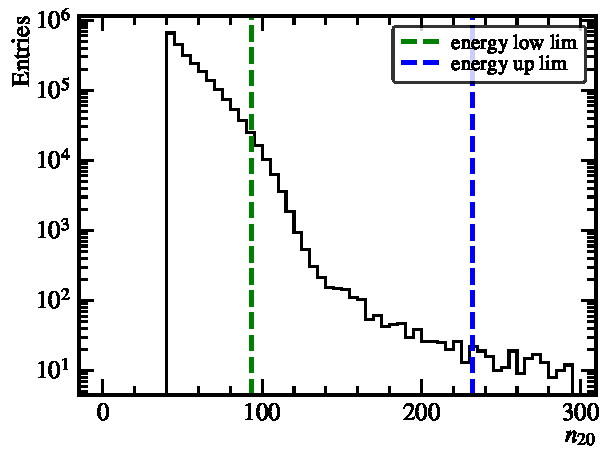
\includegraphics[width=0.5\textwidth]{solarSearch/n20Cut.pdf}
	\caption{The selection of energy of solar neutrinos.}
	\label{fig:solar_n20_select}
\end{figure}

\subsection{The position selection}
Following the energy screening, it was observed that a substantial number of events converged at the center of the detector, as shown in Fig.~\ref{fig:solar_pos_cut}. Analogous to the scenario depicted in Fig.~\ref{fig:solar_direction}, the events at the center exhibited a downward tendency. Given that the search for solar neutrinos is highly direction-dependent, rather than implementing a direction cut, we chose an additional cylindrical region at the center of the detector for screening, as illustrated in Fig.~\ref{fig:solar_pos_cut}. Our final FV cut is:
\begin{itemize}
	\item $x^2+y^2>50$~\si{m^2}
	\item $r<14$~\si{m}
\end{itemize}

\begin{figure}[htbp]
	\centering
	\begin{subfigure}{0.5\textwidth}
		\centering
		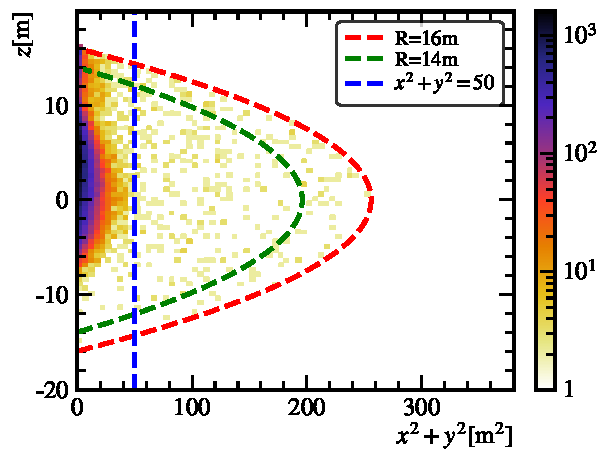
\includegraphics[width=0.9\textwidth]{solarSearch/Position_Cut.pdf}
		\label{fig:solar_pos_cut}
		% 图片宽度占子图宽度的80%
	\end{subfigure}% 
	\begin{subfigure}{0.5\textwidth}
		\centering
		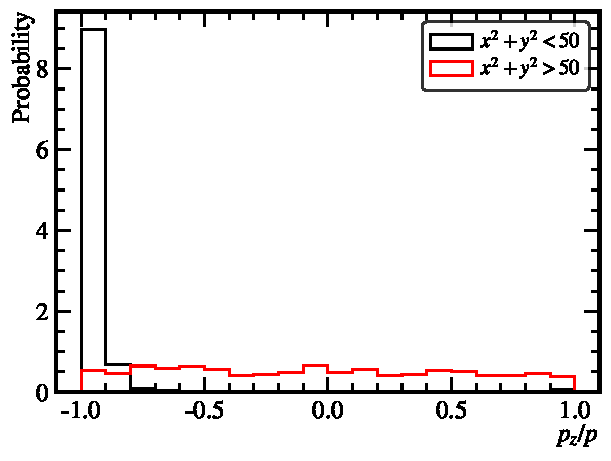
\includegraphics[width=0.9\textwidth]{solarSearch/pzp_FV.pdf}
		\label{fig:solar_direction}
	\end{subfigure}
	\caption{The position selection of solar neutrino. \subref{fig:solar_pos_cut} shows the final FV selection, while \subref{fig:solar_direction} shows direction distribution in different regions.}
	\label{fig:solar_position_cut}
\end{figure}
